\chapter{Changing the elements}
\label{sec:elements}

\textbf{Include results for CRFeMnCo to finish!}
In similar fashion to the previous sections, we here begin by presenting the mean and standard deviation of the total energy and magnetization of a set of SQSs corresponding to different high-entropy silicides of the \ch{Fesi2} unit cell. The compositions we have tested are deliberate combinations intended to investigate both the impact of manganese by replacing the element with Co or Ti, and concepts related to HEA theory such as the atomic size effect. Furthermore Co is a very common element in many stable HEA, as seen in section .., thus we include two (3?) compositions with this element to study the impact on stability and the functional properties. The results of the aforementioned alloys can be seen bellow in table 9.1, note that all compounds contain a total of 48 atoms as before.  

\begin{table}[H]
\centering
\begin{tabular}{@{}cccccc@{}}
\toprule
         & \multicolumn{2}{c}{Toten (eV)} & Enthalpy of formation &  \multicolumn{2}{c}{Mag} \\ \midrule
\ch{Cr4Fe4Co4Ni4Si32} & - 6.4655        & 0.0056     & - 12.7536       & 0.0083     & 0.0155     \\
\ch{Co4Fe4Mn4Ni4Si32} & - 6.4731        & 0.0046     & - 15.0836       & 0.0000    & 0.0000          \\
\ch{Cr4Fe4Ti4Ni4Si32} & - 6.4217        & 0.0087     & - 7.5040       & 0.0305     & 0.0293     \\
\ch{Cr4Fe4Mn4Ti4Si32} & -6.6994         & 0.0071     & - 7.3060       & 0.1142     & 0.0641     \\ 
\ch{Cr4Fe4Mn4Co4Si32} & -6.7687 		  & 0.0034     & - 13.7796      & 0.1331     & 0.0326    
\bottomrule
\end{tabular}
\caption{Summary of the total energy, enthalpy of formation and magnetization of several  composistionally different SQS high-entropy alloys based on the $\beta-$ \ch{FeSi2} unit cell.}
\end{table} 

\textbf{Maybe discuss the std of mag and relation to energy of sqs, several cases we find large differences between SQSs.}
From table 9.1 we see that the stability of the relative compositions vary greatly. By introducing cobalt to the alloys, particularly at the cost of manganese result in a large positive effect on the stability, contrary replacing either manganese or nickel with titanium significantly lowers the stability. In terms of the magnetization, the results are in line with the observations of the CFMN composition, from table 9.1 it's clear that replacing either manganese or chromium drastically reduces the magnetization of the alloys. In addition, we find indication of chromium being further significant to the magnetization than manganese as seen from the first and second compounds in table 9.1 respectively. In opposition to the study of the CFMN system we observe here a clear relation between magnetization and stability. However, we are not confident if the observed outcome is a direct consequence of the magnetization or simply a product of addition of cobalt and titanium respectively to the alloys. On the other hand, in both cases the least magnetic composition is also the most unstable, thus there is weight behind the magnetic relation to stability. \textbf{Wait for CrFeMnCoSi2 to finish}  

\begin{comment}
Bellow we include the calculated PDFs of introducing cobalt to the alloy.   
\begin{figure}[H]
	\centering
	\begin{subfigure}{\textwidth}
		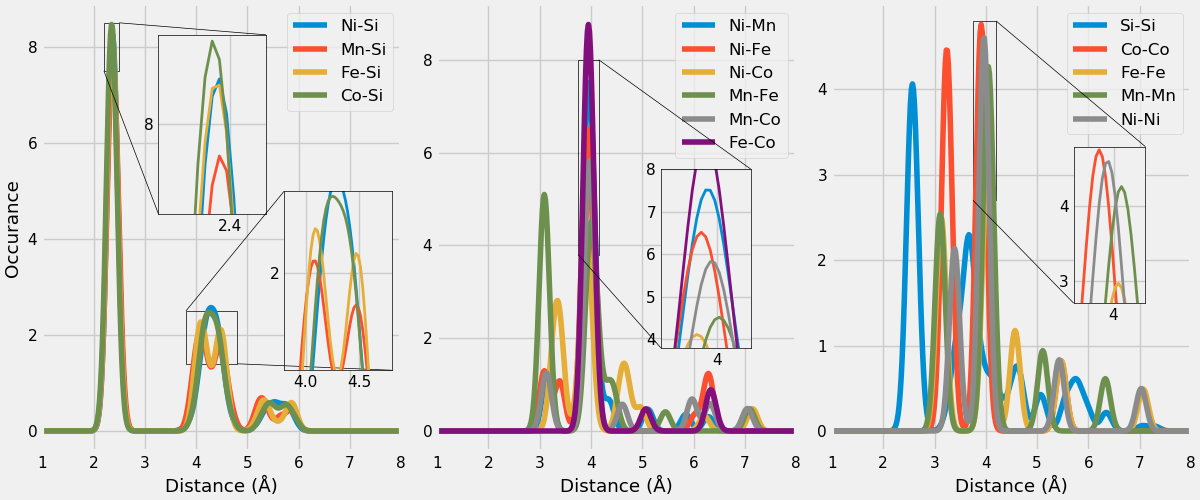
\includegraphics[width=\textwidth]{results/fesi2/composistions/cofemnni_PDF.png}
	\end{subfigure}
	\begin{subfigure}{\textwidth}
		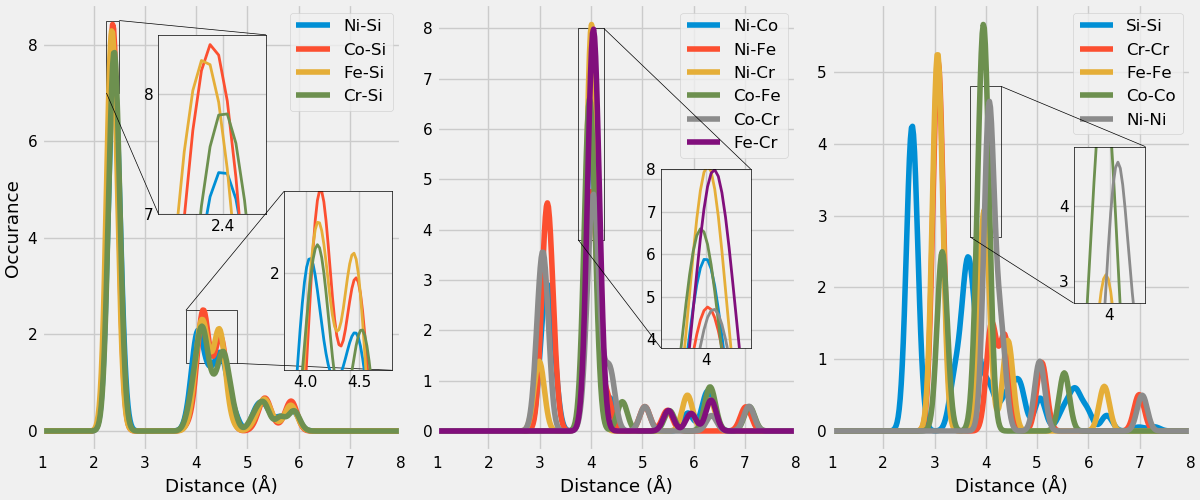
\includegraphics[width=\textwidth]{results/fesi2/composistions/crfeconi_PDF.png}
	\end{subfigure}
	\begin{subfigure}{\textwidth}
		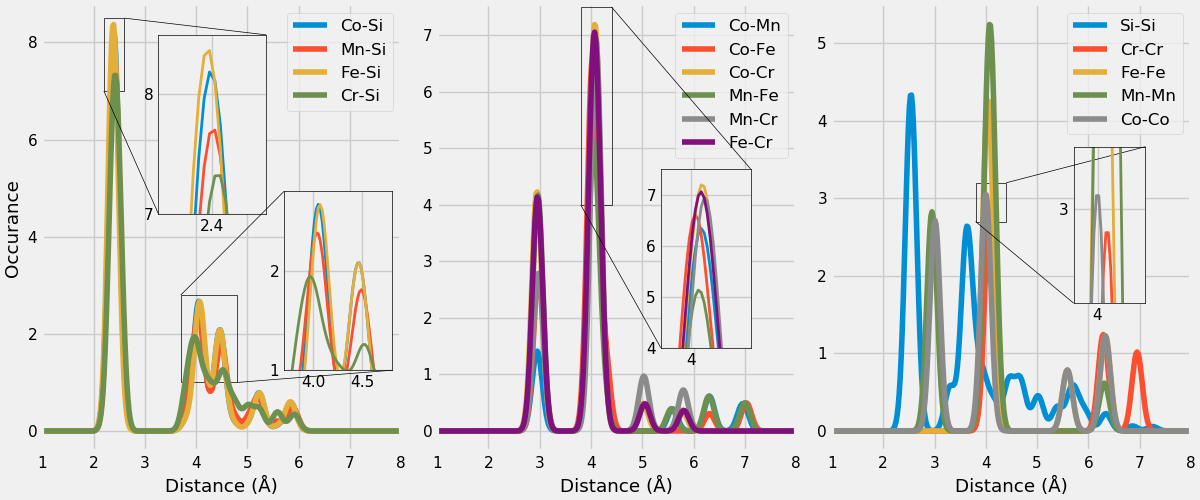
\includegraphics[width=\textwidth]{results/fesi2/composistions/crfemnco_PDF.png}
	\end{subfigure}
	\caption{Probability distribution functions of top: \ch{Co4Fe4Mn4Ni4Si32} (SQS D), middle: \ch{Cr4Fe4Co4Ni4Si32} (SQS B), bottom: \ch{Cr4Fe4Mn4Co4Si32} (SQS B)}
\end{figure}
Similarly we look at the PDFs of \ch{Cr4Fe4Mn4Ti4Si32} and \ch{Cr4Fe4Ti4Ni4Si32} bellow.
\begin{figure}[H]
	\centering
	\begin{subfigure}{\textwidth}
		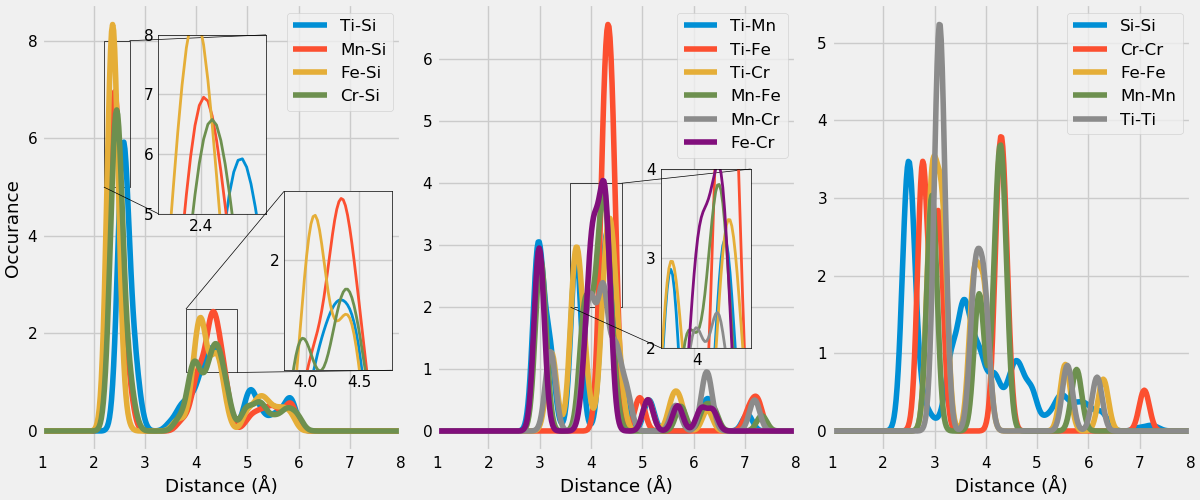
\includegraphics[width=\textwidth]{results/fesi2/composistions/crfemnti_PDF.png}
	\end{subfigure}
	\begin{subfigure}{\textwidth}
		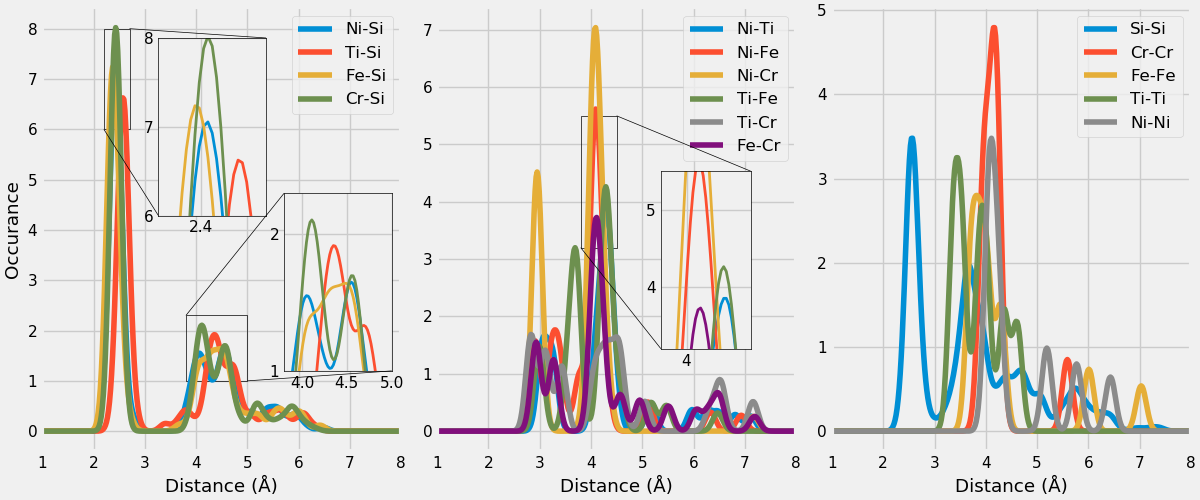
\includegraphics[width=\textwidth]{results/fesi2/composistions/crfetini_PDF.png}
	\end{subfigure}
	\caption{Probability distribution function of top: \ch{Cr4Fe4Mn4Ti4Si32} (SQS B), bottom: \ch{Cr4Fe4Ti4Ni4Si32} (SQS B))}
\end{figure}
\end{comment}  


In regards to the band gap of the compositions, we can report that a heavy majority are metals. We found no evidence of a band gap in both the CrFeCoNiSi2 and CrFeMnTiSi2 alloys across all supercells, as seen in the density of states of the two most stable SQSs of the respective compounds \textbf{Add figures}. Further also the most stable SQSs of the CrFeTiNiSi alloy point to a metal. Similarly the most stable SQSs of the CoFeMnNiSi2 alloy are clearly metals. Noteworthy of this composition however is that we find clear evidence of a narrow band gap in two SQSs (A and B). In terms of stability, these lie around the mean total energy of the set. The respective band gaps are 0.033 eV in A and 0.0058 eV in B. \textbf{Include DOS or other figures for these results.} 

\textbf{To follow is details on the gaps in A and B, is it worth to include this?}
In the density of states plotted in figure .., the band gap in A is clearly visible. On the other hand the very narrow gap in B is not as apparent, as the states around Ef contain very small nonzero values.  This could be related to the low resolution of 2500 points in the density of states as seen before, especially considering the size of the gap. In opposite to the CFMN calculations previous we here experience excellent cohesion between PBE and SCAN simulations on the band gap. With the meta-GGA functional the band gap of SQS A and B respective is 0.04 eV and the 0.003 eV. Moreover we find the identical gap transition with both functionals, which was not the case in previous endeavors with this functional. Additionally we also find that the HSE06 functional produce dissimilar results to previous experiences. In this scenario, the HSE06 functional fails to recognize the observed band gap of PBE and SCAN in both supercells. The greater number of k-points in the GGA and meta-GGA calculations offer more accurate band gaps, however lesser k-points will not result in a smaller gap, only bigger. Thus the uncertainites of previous calculations of the HSE06 functional does not apply in this case. For this reason in addition to the reputation of hybrid functionals and the lack of other factors to negatively affect the validity of the result, we find it challenging to conclude on the band gap of these structures between functionals.

\textbf{Comment PDOS figures} \\
\textbf{Make additional figures plain DOS around Ef. \\}
\begin{figure}[H]
	\centering
	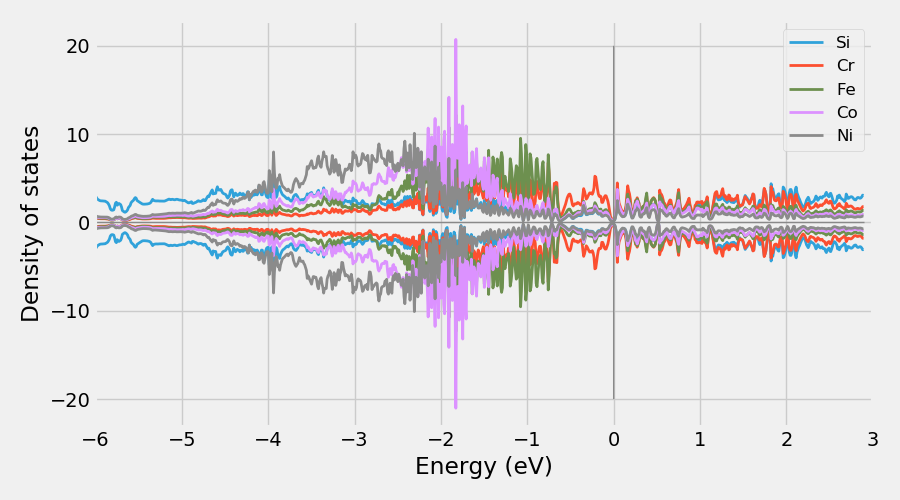
\includegraphics[width=.6\textwidth]{results/fesi2/composistions/crfeconi_PDOS_full.png}
	\caption{\ch{Cr4Fe4Co4Ni4Si32}}
\end{figure}


\begin{figure}[H]
	\begin{subfigure}{.5\textwidth}
		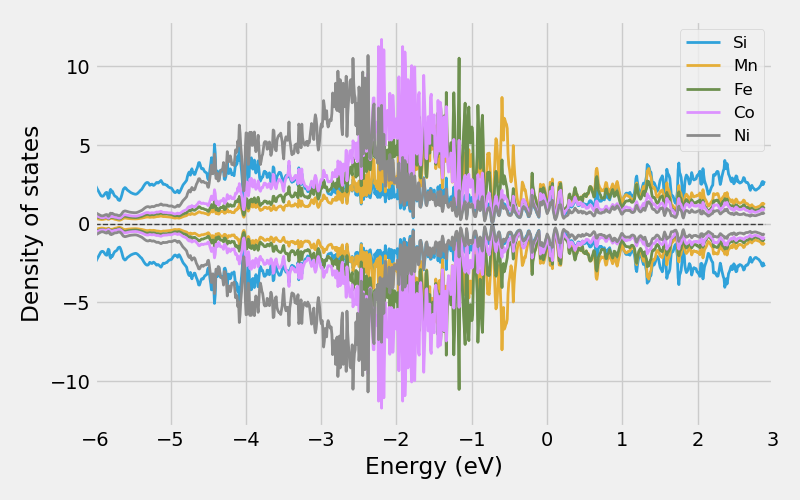
\includegraphics[width=\textwidth]{results/fesi2/composistions/cofemnni_PDOS_full.png}
		\caption{\ch{Co4Fe4Mn4Ni4Si32}}
	\end{subfigure}
	\begin{subfigure}{.5\textwidth}
		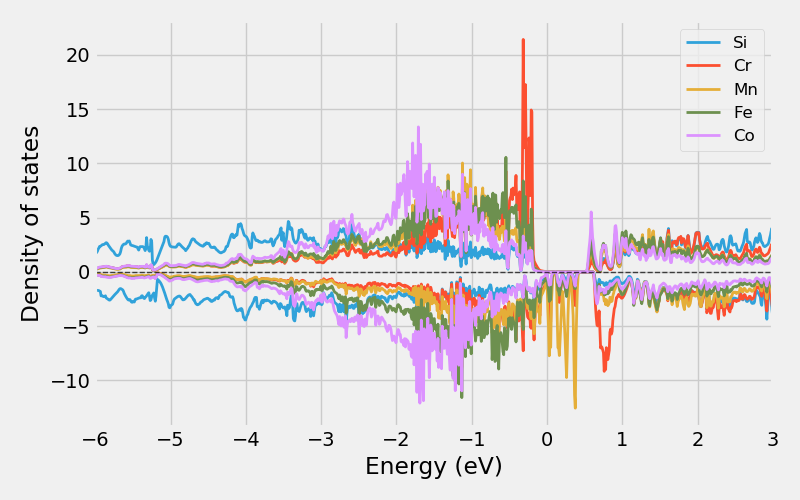
\includegraphics[width=\textwidth]{results/fesi2/composistions/crfemnco_PDOS_full.png}
		\caption{\ch{Cr4Fe4Mn4Co4Si32}}
	\end{subfigure}
\end{figure}


\begin{figure}[H]
	\begin{subfigure}{.5\textwidth}
		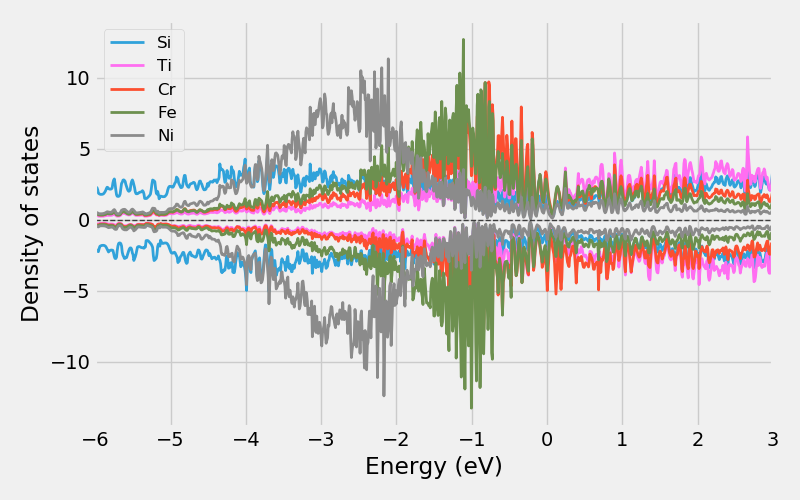
\includegraphics[width=\textwidth]{results/fesi2/composistions/crfetini_PDOS_full.png}
		\caption{\ch{Cr4Fe4Ti4Ni4Si32}}
	\end{subfigure}
	\begin{subfigure}{.5\textwidth}
		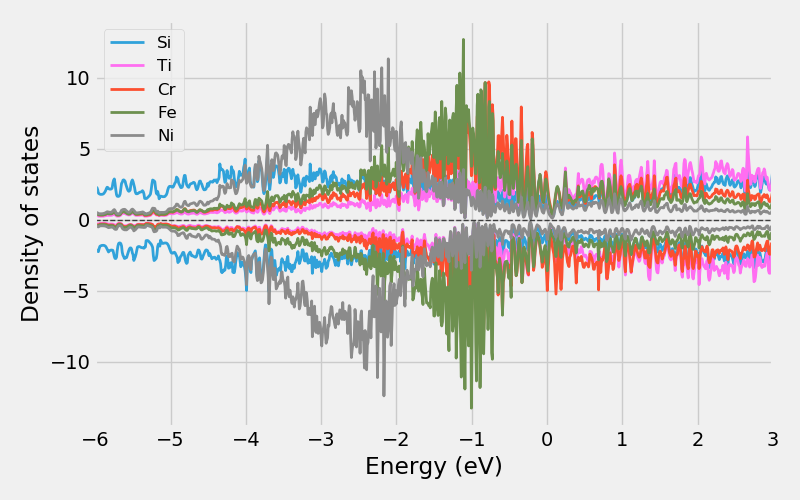
\includegraphics[width=\textwidth]{results/fesi2/composistions/crfetini_PDOS_full.png}
		\caption{\ch{Cr4Fe4Mn4Ti4Si32}}
	\end{subfigure}
\end{figure}

\textbf{Add PDFs if time maybe}